% ============================================================================
\section{Methodology}\label{sec:method}
% ============================================================================

Figure~\ref{fig:methods} summarizes the pipeline, which follows earlier large-scale tracking crawls \citep{englehardt2016online}. Every detection and classification step is a deterministic rule (URL patterns, DOM selectors, header decoding, configuration parsing), with no machine learning; Supplementary \ref*{S:sec:s-sample} gives the details.

\begin{widefig}
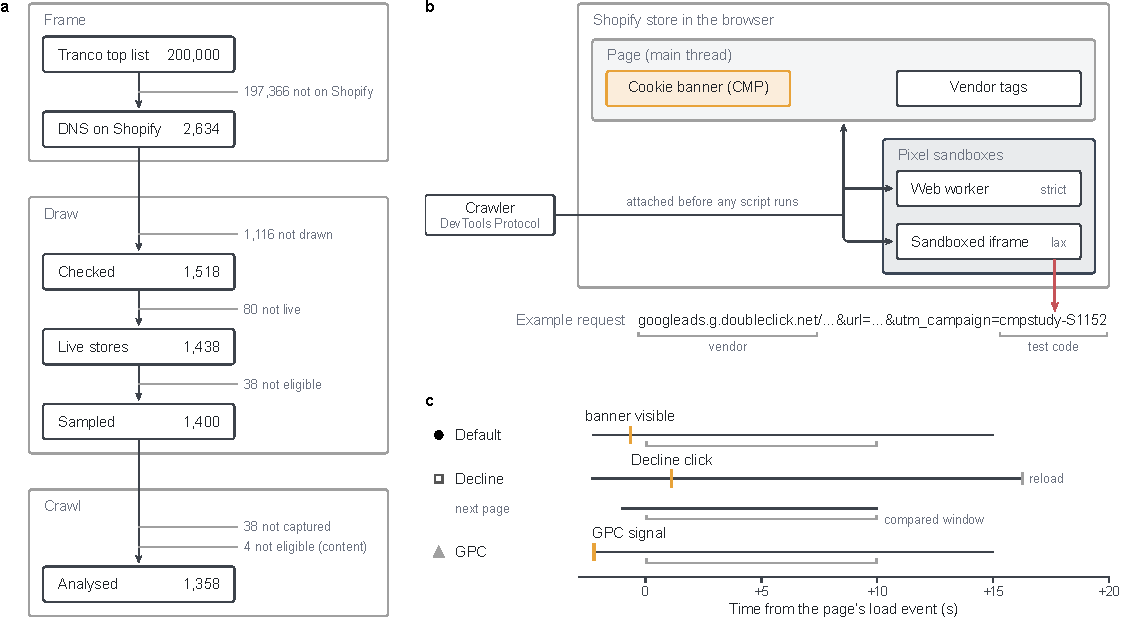
\includegraphics{fig2.pdf}
% GENERATED by paper/integrate_figures_v2.py from figures/v7/fig2/caption_fig2.tex (v2 figure caption, rendered by the figure script).
% Do not edit: change the figure script and re-run build.sh.
\caption{\textbf{We load each store three ways and label every ad request, including those sent from inside Shopify's sandboxes.} (a)~The sampling flow, top to bottom, in three phases, each in a grey outline: Frame (the sampling frame), Draw and Crawl. Each box gives a stage (left) and its count (right); grey branches with flat ends give the domains or stores removed between two stages, with their count and reason, so that each count is the one above minus its branches. Tranco top 200,000 domains; 2,634 whose domain-name system (DNS) records point to Shopify (197,366 not on Shopify by this rule); 1,518 checked: all 902 flagged domains of the three upper rank buckets and 616 of the 1,732 in the lowest, drawn in a seeded random order until its quota of eligible stores was met (the other 1,116 were not drawn); 1,438 live storefronts (80 not live); 1,400 sampled (38 not eligible: no product page, a duplicate, adult or aimed at children; Supplementary Table~\ref*{S:tab:s-exclusions}); 1,358 captured in all three base arms and analysed (38 not captured; 4 not eligible on content: adult products or aimed at children, found after the crawl and excluded for content sensitivity). Not shown: the 34 creator-linked stores of Fig.~6, a separate stratum, not counted in the 1,358. (b)~Where the crawler attaches, drawn on the store of Fig.~1a in its arrangement: a Shopify store in the browser (outer frame), with the page's main thread (light grey ground), which holds the consent-management platform's (CMP) cookie banner (amber) and the vendor tags, and, below it, the two sandboxes in which Shopify's Web Pixels Manager runs pixels (darker grey ground): a web worker (`strict' runtime) above a sandboxed iframe (`lax'). The crawler, a client of the Chrome DevTools Protocol, stands outside the browser; one bus (grey arrows) forks to every target, the page and each worker and iframe, and attaches the crawler to it before any script runs, including the sandboxes, which a CMP's script blocker in the page cannot reach (Fig.~1a). It records each request in the session of the target that sent it and labels every ad request by origin, timing, vendor and payload. Brick arrow: one captured request, the first sandboxed data beacon with our test code in the Default load of store S1152 (one row of Fig.~1c, sent before any choice; brick, as there). A Google Ads pixel sent it from the sandboxed iframe (its origin) 2,720~ms after navigation start, 53~ms before the banner became visible at 2,773~ms (its timing). The arrow lands on our test code in the request's URL below. Square brackets mark the host, which names the vendor, and the test code, cmpstudy-S1152: our pseudonymous code for the store, the value of utm\_campaign in the landing URL that the `url' parameter (the payload) carried. The request path (with the advertiser's account number), the landing page's path and all other parameter values are dropped (\ldots) so that the store cannot be identified. (c)~The three base arms as timelines under one time axis, the time from each page's load event. Each line is one page load and starts at navigation; the marker at the left is the arm's marker used throughout. Amber ticks: each arm's consent moment, named above it. Default (\mkDefault): no interaction; the banner becomes visible (the detector polls every 250~ms), and the load is observed until 15~s after its load event. Decline (\mkDecline): once the banner is visible, the Decline click on a first-layer reject control, made on 240 stores; it worked on 231 (banner gone 2~s after the click, or a refusal recorded by Shopify). The first page is observed after the click and ends at the reload (grey end tick): the same URL is loaded again in the same browser, with new sandboxes, and this next page (the row below) is observed for 10~s after its load event. Global Privacy Control (GPC, \mkGPC): the signal is set from navigation on, in every frame, worker and request. Square brackets: the equal 10~s windows on which the arms are compared (Fig.~5a), each from a load event (in Decline, the next page's), so that they share one zero. Navigation, the banner, the click, the reload and the next page's navigation vary by store and are drawn at their medians over the analysed stores: in Default, navigation 2.3~s and the banner 0.7~s before the load event (1,348 and 406 loads); in Decline (240 clicked loads), the click 1.1~s and the reload 16.3~s after the load event, and the next page's load event 1.0~s after its navigation; in GPC, navigation 2.2~s before the load event. Each base arm covers 1,358 stores. Signal, action, window and $n$ of every arm: Supplementary Table~\ref*{S:tab:s-arms}.
Panels~(a) to~(c): Drawn by figure-generation scripts written with AI assistance (Section~\ref{sec:method-ai}).}
\label{fig:methods}

\end{widefig}

\subsection{Store sample}\label{sec:method-sample}

We took the top 200,000 domains of Tranco list L5PZ4, created on 25 September 2026 \citep{lepochat2019tranco,tranco_L5PZ4}, and flagged a domain if its apex or \code{www} host had an A record in 23.227.32.0/19, the IPv4 block registered to Shopify, or a CNAME chain ending at \code{*.myshopify.com}; 2,634 domains were flagged (Fig.~\ref{fig:methods}a; Supplementary Table~\ref*{S:tab:s-buckets}). A check after the crawl puts the rule's recall at about 83\% (bucket-wise bounds 48--96\%) but only 23\% in the top bucket, and storefronts on \code{shop.} or \code{store.} subdomains, an estimated 1,828 in the top 200,000, are outside the frame (Supplementary \ref*{S:sec:s-sample}).

We stratified by Tranco rank (1--10k, 10k--50k, 50k--100k, 100k--200k), verified all flagged domains in the three upper buckets and, in the 100k--200k bucket, domains in a seeded random order until a quota of 576 eligible stores was met, with one homepage request per site. A domain was eligible if it served a live Shopify Online Store storefront (the one that runs the WPM) with a product page and was neither adult nor aimed at children (content screen: Supplementary \ref*{S:sec:s-extended}; Section~\ref{sec:ethics}). The sample holds 1,400 stores (Supplementary Table~\ref*{S:tab:s-exclusions}); design weights (1 in the census buckets, 2.81 in the 100k--200k bucket) sum to 2,443.5, an estimate of the eligible storefronts in the frame. After the crawl, we excluded 4 of these stores from all analyses for content sensitivity: two adult-product stores that the sampling screen had missed, a toy retailer and a second store that may be aimed at children (Section~\ref{sec:ethics}). The analysed main sample therefore starts from 1,396 stores. We landed on the store's first product link.

A purposive stratum of 34 Shopify stores that YouTube creators link to with a creator-identifying token in the URL (six tokens name a single video) describes these stores only. \storeC is a mixed-audience retailer that markets to children, teenagers and adults, so it would have met the child-directed exclusion; we kept it because the study began from its public creator links, loaded only public pages, involved no data about children and did not load it again after the main crawl. We make no claim about children's data or about COPPA or the CCPA's rules for minors.

\subsection{Measurement arms and crawler}\label{sec:method-arms}

Each store was loaded under three base arms in a per-store shuffled order (Fig.~\ref{fig:methods}c; Supplementary Table~\ref*{S:tab:s-arms}):
\begin{description}
  \item[Default (\mkDefault).] No clicks: we observed until 15~s after the \code{load} event, with six passive mouse-wheel scrolls, one per second, from 2~s into that window.
  \item[Decline (\mkDecline).] We waited up to 10~s for a visible banner, took a screenshot, and clicked a reject control inside it, matched by text or CMP-specific selectors (never Accept, settings or ``Do not sell''). After 15~s we reloaded the URL in the same browser (the ``next page'') and observed for 10~s after its \code{load} event.
  \item[GPC (\mkGPC).] Every request, including worker requests, carried the \code{Sec-GPC:~1} header, and \code{navigator.globalPrivacyControl} was injected into every frame and worker before their first script (checks in Section~\ref{sec:app-validation}).
\end{description}
A seeded 20\% subsample (287 stores) repeated the Default and GPC arms, and a seeded 100-store subsample was loaded in Brave with native GPC and tracker blocking off. The URL was the landing page plus a canary token in its campaign parameters (\code{utm\_campaign=\allowbreak cmpstudy-<store\_id>}). Every load used a new browser with a new temporary profile: Playwright \citep{playwright} with Chromium's headless shell (version 149, 4,876 loads) or Brave (version 150, 100 loads, also headless), with unmodified user agents and no stealth techniques, so pages could tell that the browser was automated (Section~\ref{sec:app-validation}). The crawl ran on 26 September 2026 between 07:03 and 10:01~UTC, with at most one page load per site every 10~s.

\subsection{Instrumentation and request attribution}\label{sec:method-attr}

A client of the browser's DevTools Protocol \citep{cdp} attached automatically to every target (page, out-of-process iframe, worker) and enabled network capture before the target ran, so every request is logged in the session of the target that issued it. A request is \emph{sandboxed} if it was issued inside a worker whose URL matches the WPM's STRICT bootstrap, by a frame whose URL matches a LAX sandbox, or by a frame nested inside such a frame; sandboxed and OPEN requests are joined to their pixel's configuration entry. A rule-based map assigns each request to the advertising vendor whose endpoint \emph{receives} it (seven vendor groups) and separates library loads from data beacons. Payload flags record whether a request carries our canary, the full landing URL or a creator's token, and whether its URL carries a refusal signal of the vendor's own (Supplementary \ref*{S:sec:s-sample} and~\ref*{S:sec:s-extended}).

\subsection{Consent state, CMPs and declared policies}\label{sec:method-consent}

We decoded the \code{Server-Timing: \_cmp} string of each navigation response into the store's region default for our vantage (``allowed until choice'' when marketing is allowed, ``denied until consent'' otherwise), read Shopify's Customer Privacy API about once a second, and recorded every \code{visitorConsentCollected} event. A Decline click \emph{worked} if the banner was gone 2~s later or Shopify recorded an explicit refusal, which held for 231 of 240 clicks; Shopify \emph{recorded a refusal} if a reading after the click had \code{marketing} or \code{trackingConsent} equal to ``no''. CMPs and visible banners were detected by rules, the banners polled every 250~ms (Supplementary \ref*{S:sec:s-sample}). Each store's integration group follows the CMP that showed the banner (Table~\ref{tab:cmp-modes}): Shopify's own banner (N); a CMP that writes to Shopify (A and C); or a blocker-only, unknown or absent CMP (B and X). For Pandectes, OneTrust and Cookiebot the store-specific blocklist is readable in the page, and we recorded for every ad vendor on it whether it was declared blocked before any choice (Supplementary \ref*{S:sec:s-cmp}).

\subsection{Outcomes}\label{sec:method-outcomes}

The primary outcome is store-level: whether at least one \emph{sandboxed ad request} (a data beacon or a library load from a STRICT worker, a LAX iframe or a frame nested in it, to an advertising vendor) occurred in a given window. Because a pixel might ``seemingly load'' while its data gathering is suppressed \citep{truevault_apppixel}, every headline rate is also reported for data beacons only (Supplementary Fig.~\ref*{S:fig:s5}). Rates \emph{before any choice} use the Default load. \emph{After Decline}, the primary outcome is that a sandbox created on the next page sent an ad request within 10~s of its \code{load} event; Default and GPC are compared over the same 10~s. The \emph{gate audit} compares configured pixels whose declared purpose was denied at the moment with the pixels that started.

\subsection{Validation}\label{sec:method-validation}

We checked repeat-load agreement, the GPC injection in every frame and worker \citep{krumnow2022openwpm}, emulated against native GPC, and 54 seeded Decline loads and all 12 forced clicks from saved screenshots (Fig.~\ref{fig:reach}d; Supplementary Fig.~\ref*{S:fig:s4}). A later re-check crawl loaded 128 of the analysed main-sample stores once more, to audit the banner detector's recall and to log which elements a blocker neutralized on the 21 blocklist stores (Supplementary \ref*{S:sec:s-audit}).

\subsection{Statistical analysis}\label{sec:method-stats}

Store-level proportions carry Wilson 95\% confidence intervals \citep{wilson1927probable}, and headline rates also, as a sensitivity analysis, a BCa cluster bootstrap by consent tool \citep{field2007bootstrapping}, because banner behaviour is a property of the consent product. Paired differences between arms carry Newcombe's interval for paired data \citep{newcombe1998paired}, other differences his interval for independent samples \citep{newcombe1998independent}, and stratified differences are Mantel--Haenszel estimates \citep{mantel1959statistical}. Intervals for shares whose unit is not a store resample stores (a percentile bootstrap, or the Korn--Graubard interval \citep{korn1998survey}), Cohen's $\kappa$ \citep{cohen1960kappa} is read against \citet{landis1977agreement}, and Firth-penalized logistic models \citep{firth1993bias,heinze2002separation} are exploratory. The primary estimates are the three headline rates (pre-choice firing on banner stores, the fresh-page residual after Decline and the residual under GPC), the blocked-on-paper rate on stores whose CMP had not itself consented (pooled over the main sample and the expansion), and the paired difference between Decline and GPC; other intervals are descriptive and not adjusted for multiplicity (further details: Supplementary \ref*{S:sec:s-extended}). One script regenerates the analysis outputs from the saved crawl data, and an automated check traces every number in the manuscript to those outputs or, for the literature, to the cited papers.

\subsection{Round 4: blocklist expansion and a pilot beyond Shopify}\label{sec:method-r4}

A second crawl on 27 September 2026 ran the same crawler and arms, at most six concurrent browsers and at least 10~s between two loads of a site; unlike the main crawl, it fetched each site's \code{robots.txt} first and loaded a site only if it allowed the page (Section~\ref{sec:ethics}). \emph{Expansion.} Screening Tranco ranks 200,001--1,000,000 with the main sample's DNS and eligibility rules found, among 11,354 eligible storefronts, 120 whose readable Pandectes or OneTrust blocklist declared an ad vendor blocked before any choice for a California visitor or could only be settled at run time; all were loaded, 116 were captured in all three arms, and on 96 the blocklist was in force at run time. The blocked-on-paper estimands were computed by the main pipeline's own code, which reproduced every main-sample value exactly. \emph{Pilot.} We selected 80 Wix and 80 BigCommerce sites, 26 sites that send Google tags through a first-party gateway (a tag endpoint on the site's own domain), and all 8 Partytown sites and 1 Cloudflare Zaraz site that the screen found. First-party requests were attributed to a vendor only when their wire format named it, and server-side forwarding was never inferred (Supplementary \ref*{S:sec:s-r4}).

\subsection{Changes to the planned protocol}\label{sec:method-deviations}

The study had no public preregistration; the planned protocol and eight predictions about the mechanism were written in an internal note before the crawl, and Supplementary Table~\ref*{S:tab:s-predictions} reports how each fared. Three changes were made during the crawl, the largest that most loads ran at ten rather than the planned six concurrent browsers, with per-site pacing unchanged; three checks were added after the analyses (Supplementary \ref*{S:sec:s-extended}).

\subsection{Use of generative AI}\label{sec:method-ai}

During the preparation of this work the author used Anthropic's Claude to assist with writing and debugging the measurement, analysis, and figure-generation scripts. The author reviewed the code and its outputs and takes full responsibility for the content of the publication. The validation labels (the 21 content-screen decisions, the screenshot audits of 54 Decline loads and 12 forced clicks, and the blind recall audit of the 128 re-check loads) were made with the same assistance rather than by an independent human rater, so they are not an independent validation; a kit for blind re-labelling is released with the data.
